% -*- Mode:TeX -*-

%% IMPORTANT: The official thesis specifications are available at:
%%            http://libraries.mit.edu/archives/thesis-specs/
%%
%%            Please verify your thesis' formatting and copyright
%%            assignment before submission.  If you notice any
%%            discrepancies between these templates and the
%%            MIT Libraries' specs, please let us know
%%            by e-mailing thesis@mit.edu

%% The documentclass options along with the pagestyle can be used to generate
%% a technical report, a draft copy, or a regular thesis.  You may need to
%% re-specify the pagestyle after you \include  cover.tex.  For more
%% information, see the first few lines of mitthesis.cls.

%\documentclass[12pt,vi,twoside]{mitthesis}
%%
%%  If you want your thesis copyright to you instead of MIT, use the
%%  ``vi'' option, as above.
%%
%\documentclass[12pt,twoside,leftblank]{mitthesis}
%%
%% If you want blank pages before new chapters to be labelled ``This
%% Page Intentionally Left Blank'', use the ``leftblank'' option, as
%% above.

\documentclass[11pt,twoside]{mitthesis}
\usepackage{lgrind}
%% These have been added at the request of the MIT Libraries, because
%% some PDF conversions mess up the ligatures.  -LB, 1/22/2014
\usepackage{cmap}
\usepackage[T1]{fontenc}
\usepackage{amsmath, amssymb, amsthm}
\usepackage{listings}
\usepackage{xcolor}
\usepackage{graphicx}
\usepackage{url}
\usepackage{todonotes}
\usepackage{mdframed}

\newcommand{\afunc}[1]{\operatorname{\mathsf{#1}}}

\theoremstyle{definition}
\newtheorem{definition}{Definition}[section]

\lstdefinestyle{base}{
  language=python,
  basicstyle=\ttfamily\footnotesize,
  numbers=none,
  frame=single,
  stepnumber=1,
  rulecolor=\color{black},
  breaklines=true,
  captionpos=b
}

\renewcommand{\lstlistingname}{Figure}

\newcommand{\SV}{\afunc{SV}}
\newcommand{\Com}{\afunc{Com}}
\newcommand{\ComSV}{\afunc{ComSV}}
\pagestyle{plain}

\graphicspath{ {images/} }

%% This bit allows you to either specify only the files which you wish to
%% process, or `all' to process all files which you \include.
%% Krishna Sethuraman (1990).

% \typein [\files]{Enter file names to process, (chap1,chap2 ...), or `all' to
% process all files:}
% \def\all{all}
% \ifx\files\all \typeout{Including all files.} \else \typeout{Including only \files.} \includeonly{\files} \fi

\begin{document}

% -*-latex-*-
%
% For questions, comments, concerns or complaints:
% thesis@mit.edu
%
%
% $Log: cover.tex,v $
% Revision 1.8  2008/05/13 15:02:15  jdreed
% Degree month is June, not May.  Added note about prevdegrees.
% Arthur Smith's title updated
%
% Revision 1.7  2001/02/08 18:53:16  boojum
% changed some \newpages to \cleardoublepages
%
% Revision 1.6  1999/10/21 14:49:31  boojum
% changed comment referring to documentstyle
%
% Revision 1.5  1999/10/21 14:39:04  boojum
% *** empty log message ***
%
% Revision 1.4  1997/04/18  17:54:10  othomas
% added page numbers on abstract and cover, and made 1 abstract
% page the default rather than 2.  (anne hunter tells me this
% is the new institute standard.)
%
% Revision 1.4  1997/04/18  17:54:10  othomas
% added page numbers on abstract and cover, and made 1 abstract
% page the default rather than 2.  (anne hunter tells me this
% is the new institute standard.)
%
% Revision 1.3  93/05/17  17:06:29  starflt
% Added acknowledgements section (suggested by tompalka)
%
% Revision 1.2  92/04/22  13:13:13  epeisach
% Fixes for 1991 course 6 requirements
% Phrase "and to grant others the right to do so" has been added to
% permission clause
% Second copy of abstract is not counted as separate pages so numbering works
% out
%
% Revision 1.1  92/04/22  13:08:20  epeisach

% NOTE:
% These templates make an effort to conform to the MIT Thesis specifications,
% however the specifications can change.  We recommend that you verify the
% layout of your title page with your thesis advisor and/or the MIT
% Libraries before printing your final copy.
\title{Exploring Constraint Removal Motion Planners}

\author{Amruth Venkatraman}
% If you wish to list your previous degrees on the cover page, use the
% previous degrees command:
%       \prevdegrees{A.A., Harvard University (1985)}
% You can use the \\ command to list multiple previous degrees
%       \prevdegrees{B.S., University of California (1978) \\
%                    S.M., Massachusetts Institute of Technology (1981)}
%\prevdegrees{S.B., Massachusetts Institute of Technology (2014)}

\prevdegrees{B.S., Massachusetts Institute of Technology (2015)}
\department{Department of Electrical Engineering and Computer Science}

% If the thesis is for two degrees simultaneously, list them both
% separated by \and like this:
% \degree{Doctor of Philosophy \and Master of Science}
\degree{Master of Engineering in Electrical Engineering and Computer Science}

% As of the 2007-08 academic year, valid degree months are September,
% February, or June.  The default is June.
\degreemonth{June}
\degreeyear{2016}
\thesisdate{May 20, 2016}

%% By default, the thesis will be copyrighted to MIT.  If you need to copyright
%% the thesis to yourself, just specify the `vi' documentclass option.  If for
%% some reason you want to exactly specify the copyright notice text, you can
%% use the \copyrightnoticetext command.
%\copyrightnoticetext{\copyright IBM, 1990.  Do not open till Xmas.}

% If there is more than one supervisor, use the \supervisor command
% once for each.
\supervisor{Prof. Tom\'{a}s Lozano-P\'{e}rez}{}

% This is the department committee chairman, not the thesis committee
% chairman.  You should replace this with your Department's Committee
% Chairman.
\chairman{Dr. Christopher Terman}{Chairman, Masters of Engineering Thesis Committee}

% Make the titlepage based on the above information.  If you need
% something special and can't use the standard form, you can specify
% the exact text of the titlepage yourself.  Put it in a titlepage
% environment and leave blank lines where you want vertical space.
% The spaces will be adjusted to fill the entire page.  The dotted
% lines for the signatures are made with the \signature command.
\maketitle

% The abstractpage environment sets up everything on the page except
% the text itself.  The title and other header material are put at the
% top of the page, and the supervisors are listed at the bottom.  A
% new page is begun both before and after.  Of course, an abstract may
% be more than one page itself.  If you need more control over the
% format of the page, you can use the abstract environment, which puts
% the word "Abstract" at the beginning and single spaces its text.

%% You can either \input (*not* \include) your abstract file, or you can put
%% the text of the abstract directly between the \begin{abstractpage} and
%% \end{abstractpage} commands.

% First copy: start a new page, and save the page number.
\cleardoublepage
% Uncomment the next line if you do NOT want a page number on your
% abstract and acknowledgments pages.
% \pagestyle{empty}
\setcounter{savepage}{\thepage}
\begin{abstractpage}
% $Log: abstract.tex,v $
% Revision 1.1  93/05/14  14:56:25  starflt
% Initial revision
%
% Revision 1.1  90/05/04  10:41:01  lwvanels
% Initial revision
%
%
%% The text of your abstract and nothing else (other than comments) goes here.
%% It will be single-spaced and the rest of the text that is supposed to go on
%% the abstract page will be generated by the abstractpage environment.  This
%% file should be \input (not \include 'd) from cover.tex.

% no more than 150 words
\emph{TODO}

\end{abstractpage}

% Additional copy: start a new page, and reset the page number.  This way,
% the second copy of the abstract is not counted as separate pages.
% Uncomment the next 6 lines if you need two copies of the abstract
% page.
% \setcounter{page}{\thesavepage}
% \begin{abstractpage}
% % $Log: abstract.tex,v $
% Revision 1.1  93/05/14  14:56:25  starflt
% Initial revision
%
% Revision 1.1  90/05/04  10:41:01  lwvanels
% Initial revision
%
%
%% The text of your abstract and nothing else (other than comments) goes here.
%% It will be single-spaced and the rest of the text that is supposed to go on
%% the abstract page will be generated by the abstractpage environment.  This
%% file should be \input (not \include 'd) from cover.tex.

% no more than 150 words
\emph{TODO}

% \end{abstractpage}

\cleardoublepage

% \section*{Acknowledgments}
% \begin{singlespace}

% \end{singlespace}

%%%%%%%%%%%%%%%%%%%%%%%%%%%%%%%%%%%%%%%%%%%%%%%%%%%%%%%%%%%%%%%%%%%%%%
% -*-latex-*-

\pagestyle{plain}
  % -*- Mode:TeX -*-
%% This file simply contains the commands that actually generate the table of
%% contents and lists of figures and tables.  You can omit any or all of
%% these files by simply taking out the appropriate command.  For more
%% information on these files, see appendix C.3.3 of the LaTeX manual.
\tableofcontents
\newpage
\listoffigures
\newpage
\listoftables


%% This is an example first chapter.  You should put chapter/appendix that you
%% write into a separate file, and add a line \include{yourfilename} to
%% main.tex, where `yourfilename.tex' is the name of the chapter/appendix file.
%% You can process specific files by typing their names in at the
%% \files=
%% prompt when you run the file main.tex through LaTeX.
\chapter{Introduction} \label{intro}
An essential component in autonomous robotics is a planner. These invisible systems are used to make sense of the task to be performed. This involves an encoding of the world (including objects in the world and the dynamics of the physical robot). 


\section{A Brief History of Voting Systems} \label{intro:history}

\section{The Rise of Electronic Voting} \label{intro:evoting}

\section{Conclusion} \label{intro:conclusion}


\chapter{Existing Motion Planning Techniques} \label{chap:traditional_techniques}
In this chapter, we look at an overview of recent developments in motion planning. We go over their advantages and limitations. Since most motion planning algorithms incorporate randomness, with some probability they will at some point perform worse than other algorithms. Consequently, we are interested in how often they perform well to measure their robustness.

\section{Traditional Motion Planning Techniques} \label{planning:techniques}
We look at two classes of traditional planners: multi-query and single-query. The planning techniques discussed in this section only look for feasible paths --- those without collisions.

\subsection{Multi-query Planners}
Multi-query planners are meant to support multiple queries for paths between start and goal configurations in the same environment. This means that the parameters of the world are unchanging, including the obstacles, their location, and the size of the world. The multiple query nature of the planner means the planner is designed and optimized to build a data structure that will prove useful regardless of the specified start and goal configurations for a planning instance. This can mean that prior to even computing any paths, the planner must spend time on computation to accumulate this useful information.

\subsubsection{Probabilistic Roadmap}
The probabilistic roadmap (PRM) is one such multi-query planner \cite{kavraki:prm}. The PRM works in two phases - the learning phase and the query phase. The learning phase works by initializing a graph $G=(V,E)$ and growing it with a twofold process. 

The first step is the construction step in which we sample points and connect them. Specifically, we sample a random configuration $c$ from free space and add it to $G$. Then using a selection strategy, we choose some nodes from $V$ to attempt connection with $c$. If the direct path from $c$ to each of these nodes is collision free, add this edge to $E$. The second step is the expansion step which helps achieve good exploration in "difficult" areas. We do this by sampling points with a distribution proportional to the need to explore each area, which is approximated by a heuristic. Then given one of these vertices, we choose an arbitrary direction and extend in that direction. Whenever an obstacle is hit, we pick another random direction and repeat this with some limit. Finally this final configuration is connected similarly in the construction step. 

By the end of the learning phase, the PRM is ready for querying. As soon as a path is found from each of the specified start and goal configurations to a vertex in $G$, a path can be constructed for the entire trajectory that is already known to be collision free. This is helpful as it can reduce the number of expensive collision checks that need to be done for a particular planning problem. 

The PRM is an effective method for multi-queries because it leverages the fact that the world does not change, so a collision free trajectory at this instant will be collision free at a future time as well. However, this very strength is a limitation, as it can't be used efficiently in a planner that moves obstacles. The time spent pre-computing trajectories will only be useful that one time and can provide no further benefit.

\subsection{Single-query Planners}
Single-query planners are valuable tools in scenarios where we expect the world to change over time, either because obstacles are moving or dynamics of the robot are changing (perhaps the robot is now holding something). Since we do not benefit from pre-computation, a single-query planner must be efficient at answering a particular planning question. Below we discuss advances made in this sub-field of single-query planners that are still relevant today.

\subsubsection{Rapidly-Exploring Random Trees} \label{planning:rrt}
The rapidly-exploring random tree (RRT) is a randomized data structure that was designed with few tunable parameters and heuristics \cite{lavalle:rrt}. The holonomic variant of the procedure is shown in Algorithm \ref{alg:rrt}.

{\singlespacing{
\begin{algorithm}
\caption{RRT}
\label{alg:rrt}
\begin{algorithmic}[1]
\Function{Generate RRT}{$x_{init}$, $K$}
\State $T$.init($x_{init}$)
\For{k = 1 to $K$}
\State $x_{rand} \gets$ \Call{Random Sample}{}
\State $x_{near} \gets$ \Call{Nearest}{$x_{rand}, T$}
\State $x_{new} \gets$ \Call{Stopping Configuration}{$x_{near}, x_{rand}$}
\State $T$.add\_vertex($x_{new}$)
\State $T$.add\_edge($x_{near}, x_{new}$)
\EndFor
\State Return $T$
\EndFunction
\end{algorithmic}
\end{algorithm}
}}

This data structure grows by iteratively sampling from a configuration space. It then finds the closest data point $x_{near}$ currently in our tree data structure $T$. Given these two configurations, we attempt to find a stopping configuration that is an extension in the direction from $x_{near}$ to $x_{rand}$. This procedure performs collision checking along the vector to maintain the invariant that any vertices and edges added to $T$ are collision free. If a collision free stopping configuration $x_{new}$ is found, we augment $T$ wit an edge from $x_{near}$ to $x_{new}$. To use the RRT in a motion planning scenario where we plan from $x_1$ to $x_2$, we simply instantiate the RRT with $x_{init} = x_1$ and check if $x_{new}$ is sufficiently close to $x_2$. If such an $x_2$ is found, then a path can be reconstructed using $T$.

The RRT has some nice properties. First, the RRT is likely to explore unexplored areas in the configuration space given a reasonable sampling strategy (e.g. uniform sampling). In the case of uniform sampling, the probability of an existing configuration being expanded is proportional to the size of its corresponding Voronoi region. Because the largest Voronoi regions are on the frontier of searched space, the tree will grow towards unexplored area. Second, the distribution in the RRT data structure approaches the sampling distribution as the RRT is grown. The last and arguably most important aspect is that, like the PRM, the RRT is probabilistically complete, meaning that the probability that a solution is found (if it exists) approaches 1 as the amount of time spent on the RRT plan increases. A very significant drawback of this algorithm is that this algorithm \emph{cannot} determine that there does not exist a solution. It can try indefinitely to find a solution.

\subsubsection{Goal Biased RRT} \label{planning:goal-bias}
While the aforementioned RRT motion planning algorithm is probabilistically complete, it does not provide useful bounds on how \emph{fast} it can find a solution given that one exists. As the RRT name suggests, it randomly explores the state space, eventually exploring the entire space in the limit. In a motion planning setting we know exactly where we want a path to terminate, namely the goal. A simple, yet powerful idea was to modify the sampling strategy to include a goal bias \cite{lavalle:rrt}. That is, with some small probability $p$ we "sample" the goal and with probability $1-p$ we sample from the original strategy. The choice of $p$ affects the prioritization of state space exploration versus greedy search. A lower $p$ defers to the standard RRT, with $p=0$ being exactly the original RRT. A higher value of $p$ will stretch the current tree towards the goal and more strongly guide the expansion. Goal biasing is often a good choice since in single-query planning we are interested in some path rather than a complete understanding of the reachability of the space.

\subsubsection{Bidirectional RRT} \label{planning:birrt}
The bidirectional RRT method was proposed by Kuffner and Lavalle in 2005 as a means to speed up the RRT algorithm \cite{lavalle:birrt}. It is based on a similar principle as the goal biased RRT in that we can guide the direction of the growth of the RRT. However, instead of growing a single tree, we can instantiate two RRTs and help them grow towards each other. Doing so can help the planner find solutions more quickly, as in the case when there are bug traps in the configuration space \cite{lavalle:planning}. To encourage the rapidly exploring nature of the RRT, the bi-RRT simply maintains that the difference between tree sizes never gets too large. The algorithm pseudocode is shown in Algorithm \ref{alg:birrt}.

{\singlespacing{
\begin{algorithm}[t]
\caption{Bidirectional RRT}
\label{alg:birrt}
\begin{algorithmic}[1]
\Function{ConstructBiRRT}{$q_s,q_g$}
\State $T_a$.init($q_s$)
\State $T_b$.init($q_g$)
\For{k = 1 to $K$}
    \State $q_s \gets$ \Call{Random Sample}{}
    \State $q_{near} \gets$ \Call{Nearest}{$T_a, q_s$}
    \State $q_n \gets$ \Call{Stopping Configuration}{$q_{near}, q_s$}
    \If{$q_{near} \ne q_n$}
        \State $T_a$.add\_vertex($q_n$)
        \State $T_a$.add\_edge($q_{near}, q_n$)
        \State $q_{near}' \gets$ \Call{Nearest}{$T_b, q_n$}
        \State $q_n' \gets$ \Call{Stopping Configuration}{$q_{near}', q_n$}
        \If{$q_{near}' \ne q_n'$}
            \State $T_b$.add\_vertex($q_n'$)
            \State $T_b$.add\_edge($q_{near}', q_n'$)
        \EndIf
        \If{$q_n = q_n'$}
            \State Return SOLUTION
        \EndIf
    \EndIf
    \If{$|T_a| > |T_b|$}
        \State SWAP($T_a, T_b$)
    \EndIf
\EndFor
\State Return FAILURE
\EndFunction
\end{algorithmic}
\end{algorithm}
}}

\section{The MCR Algorithm}
In this section we describe the Minimum Constraint Removal (MCR) algorithm as formulated by Hauser (for the formal problem statement see section \ref{intro:statement}). The discussion that follows draws heavily from Hauser's description \cite{hauser:mcr}. MCR is the first algorithm we discuss that tolerates collisions while searching for paths. We go into a more extensive description and analysis of MCR as we are interested in the shortcomings of this algorithm.

\subsection{Methods of Solving the MCR Problem} \label{mcr:solving}
Hauser proposed two types of solutions employing classic search techniques: an exact search method (best first search) and a close approximation that should generally run faster (greedy search).

\subsubsection{Best First Search}
This method is guaranteed to eventually find $S^{*}$. In this method, states are tuples of configuration and covers $(v, S_v)$, where $S_v$ is the cover of some path from $s \rightarrow v$. There are many such tuples for every node $v$ in the graph. We search through the graph beginning with the start node and perform best-first search using the size of the covers as the distance metric. To expand from $a$ to $b$, for two such connected vertices, we set $S_b = S_a \bigcup C[b]$. Because we maintain all possible covers for each vertex, we guarantee that the minimum constraint removal will be found. For a world with $m$ obstacles, since each configuration can have $2^m$ different covers, the total state space is $O(|E|2^m)$, making this approach infeasible.

\subsubsection{Greedy Search}
Greedy search operates much in the way that best first search does except in the enumeration of states. Rather than keeping all possible $2^m$ covers per node, we instead only maintain a cover that has the lowest size. When we expand the graph from $a$ to $b$, we re-evaluate the minimum cover $S_b$ and then update the covers of the neighbors of $b$ as necessary. Since each node is now only expanded once, the runtime is now reduced to $O(|E|m)$. In fact, if the configurations for which $O_i$ is in their covers form a connected subsequence for the found path for all $O_i \in S_g$, then $S_g = S^{*}_g$. This will often be the case --- greedy search is often as good as exact search.

\subsection{MCR Planner Details}
\subsubsection{Approximating Connectivity}
In the prior discussion, we assumed that we were already provided a graph $G$ consisting of configurations for a robot. In practice, we must construct this ourselves. We want $G$ to accurately approximate the connectivity of the configuration space, where connectivity is a function of how collision-free the space is. That is, the less cluttered the configuration space is, the more connected the space is. To formalize this notion of reachability we use $(G,k)$ reachability.

{\bf{Definition}}: A node $q$ is $(G,k)$ reachable if there is a path from a start node $s$ to $q$ with a cover at most $k$. 

The MCR planner grows $G$ in the fashion of a PRM. We repeatedly sample points randomly in our configuration space and attempt to connect them to nearby points specified by some distance metric. We also incorporate techniques from rapidly exploring random graphs (RRGs) which prioritize rapid exploration of $(G,k)$ reachable space. Specifically, when sampling a point and looking for points to connect it to, we consider only those that are $(G,k)$ reachable. This ensures that we are expanding from the \emph{exploration limit}. This way we can expand the connectivity of our $(G,k)$ reachable space. The combination of these techniques improves the connectivity of $G$ and the approximation of the real connectivity. 

By examining the psueodocode in Algorithm \ref{alg:mcr}, we see that we increment $k$ every $N_{raise}$ steps ($N_{raise}$ can be chosen as needed based on the size of the problem). This ensures that we get good connectivity for a particular exploration limit before trying to search for less accessible configurations. Having good connectivity for lower $k$ helps improve the accuracy of the approximation to the real connectivity. 

\subsubsection{Weighted MCR}
The weighted MCR problem can be trivially extended from the original formulation by defining the minimum constraint removal to be the minimum sum of weights for obstacles in the cover of a best path from the start to goal configuration. We can further emulate immovable obstacles by assigning them "infinite" weight such that the MCR planner will never plan a path through these obstacles if possible. 

Throughout this paper, we will use the notation $|S|$ to refer to the cover size in both the unweighted and weighted constraint removal problem; from the planning problem it is clear whether this refers to the cardinality of $S$ or the sum of the weighted obstacles in $S$. 

\subsubsection{Implementation Specifics}
The pseudocode in Algorithm \ref{alg:mcr} is largely similar to Hauser's original MCR formulation. We introduce an explicit exit condition for the MCR algorithm and modify the \textproc{Extend Toward} to fail if the original extension fails. 

%\begin{figure}[H]
{\singlespacing{
\begin{algorithm}[t]
\caption{Minimum Constraint Removal}
\label{alg:mcr}
\begin{algorithmic}[1]
\Function{MCR}{$q_s, q_g$}
\State $S_{min} \gets$ \Call{EdgeCover}{$q_s, q_g$} 
\State $k \gets |$Cover$(q_s) \bigcup$ Cover$(q_g)|$ 
\State $G \equiv (V,E) \gets ({q_s \rightarrow q_g})$
\While{iteration count < $N_{raise} \times (S_{min} + tolerance)$}
\State \Call{Expand Roadmap}{$G,k$}
\State Compute the minimum explanations $S_G(q)$ for all $q \in V$
\State $S_{min} \gets S_g$
\State Every $N_{raise}$ step, $k \gets k + 1$
\If{$k \ge |S_{min}|$}
    \State $k \gets |S_{min}| - 1$
\EndIf
\EndWhile
\EndFunction
\\
\Function{Expand Roadmap}{$G,k$}
\State $q_d \gets Sample()$
\State Let $q_n \gets$ \Call{Closest}{$G,k, q_d$}
\State $q \gets$ \Call{Extend Toward}{$q_n, q_d, \delta, k$}
\If{$q$ is not $None$}
    \State Let ${q_1, q_2, ..., q_n} \gets$ \Call{Neighbors}{$G,q$}
    \For {$i = 1,2,....n$}
    \If{$d(q_i,q) < \delta$}
    \State Add $q_i \rightarrow q$ to $E$
    \EndIf
    \EndFor
\EndIf
\EndFunction
\\
\Function{Closest}{$G,k,q$}
\State Return $\argmin\limits_{q_i \in V} d(q, q_i)$
\EndFunction
\\
\Function{Neighbors}{$G,q$}
\State $Distances \gets []$
\For {$i = 1,2, ..., |V|$}
\State $Distances \gets Distances + [(d(q, q_i), i)]$
\EndFor
\State Sort($Distances$)
\State Return first $m$ neighbors in $Distances$
\EndFunction
\\
\Function{Extend Toward}{$q_i, q, \delta, k$}
\State $q' \gets q_i + min(\frac{\delta}{d(q_i, q)}, 1)(q- q_i)$
\State Return $q'$ if $|S_q \bigcup$ \Call{EdgeCover}{$q_i,q'$}$| <= k$ else $None$
\EndFunction
\end{algorithmic}
\end{algorithm}
}}

The MCR algorithm follows a straightforward loop. In the initialization, we compute an upper bound on $S^{*}_g$ since $S^{*}_g$ can be no worse than the straight path from $s \rightarrow g$. Next we set $k$ to the union of the covers at $s$ and $g$ since this is at most the initial $S_{min}$ value. Then we initialize our graph and begin the task of growing and measuring connectivity in lines 5-11. 

The subroutine \textproc{Expand Roadmap} first generates a random configuration $q_d$. It then finds the closest $(G,k)$ reachable node $q_n$. Similar to RRT growth, we extend $q_n$ towards $q_d$ up to some distance tolerance $\delta$. If this new configuration $q'$ isn't within the $k$ exploration limit, we abandon and restart the for loop of MCR. Now that we have a new vertex $q'$ to add to $G$, we choose neighbor candidates. As mentioned before, we incorporate the RRG strategy and connect $q'$ to up to $m$ of the nearest configurations as long as they are at most $\delta$ away \cite{karaman:rrg}. By construction in \textproc{Extend Toward}, we know that at least one neighbor will be within $\delta$ ($q_n$). 

Finally, given our expanded graph, we can compute the minimum explanations (the minimum $(G,k)$ reachabilities) for all nodes. This is exactly the procedure described in Section \ref{mcr:solving}. Since speed is primarily what we are concerned with (at the cost of complete correctness), we use the greedy method.

While we increment $k$ every $N_{raise}$ steps, we cap it to be one less than $S_{min}$, as it is unhelpful to raise our exploration limit higher than what we know is necessary. 

While the algorithm seems simple, there are some subtleties that help it succeed. We have emphasized the importance of respecting the exploration limit $k$. When we look for candidate nodes to connect a sample to, we only consider those that are $(G,k)$ reachable since we want to improve our estimation of the connectivity of $(G,k)$ reachable space. However, the next procedure \textproc{Neighbors}($G,q$) does not consider $k$. This appears to be inconsistent with the goal of maintaining the $k$ frontier, as we would now connect $q'$ to nodes that are not necessarily contained within the limit. However, this is essential to \emph{improving} $(G,k)$ reachability.

\subsection{MCR algorithm benefits and disadvantages}
The MCR algorithm succeeds where traditional planning fails. RRTs and other strategies can search forever looking for a path from a start configuration to a goal configuration. Until such a path is found, there is no deliverable progress. Hauser's MCR technique does not suffer from this weakness because it is an \emph{any-time} algorithm, meaning the algorithm can be terminated at any point and the minimum cover path thus far can be reconstructed. A downside is that in many cases, the cover of a best path is equal to the weight of the union of the two covers at the start and goal configurations; this is the solution that MCR starts with. However, it is not clear that it can terminate instead of continuing to iterate. This is a problem of looking for paths that tolerate some collisions -- the cover of some best path is not known a priori. We instead must assume that after some period of looking for better paths, if none is found, there is no better path. For this reason we modify the original formulation of MCR to run for a number of iterations that is an increasing linear function of the best path cover found thus far.

Another difficulty the MCR algorithm faces is in its frontier expansion strategy. If a best path from the start to goal configurations has a high weight cover of $w_h$, then until the MCR algorithm goes through $N_{raise} * w_h$ expansion steps (assuming a collision-free start and goal) this path can never be found. In fact, if we were to enumerate all possible unique covers, any $k$ considered between these values are unhelpful to finding paths. It helps to build a more dense graph, but this dense graph can be limited in its exploration of the configuration space and, depending on the distribution of obstacle weights, may spend excessive time developing these frontiers.


\chapter{Collision Supported Path Planning}
In this chapter, we will look at a number of algorithms we propose for finding paths that are tolerant of collisions. These approaches will favor different strategies for finding these paths such as finding optimal paths versus computation time (or a combination of these). The discussion on algorithm performance will be addressed in the following chapter. The different algorithms that will be discussed are as follows.

\begin{enumerate}
\item Obstacle ignorant Bi-directional RRT
\item Bi-directional RRT with greedy object removal
\item Bi-directional RRT with probabilistic object removal
\item Repeated Bi-directional RRT with object removal
\item Bi-directional RRT object with removal and adding
\end{enumerate}

Note that all of the RRT variants are actually bi-RRT variants but for conciseness we will just refer to them as RRT variants.

\section{Obstacle Ignorant RRTs}
In this section we will describe a simple alternative to the traditional RRT that enables it to find paths that tolerate collisions. In particular this algorithm favors finding some path very quickly and does not prioritize minimizing the total path cover. We will shorthand this planner as OIRRT (obstacle ignorant RRT).

\subsection{OIRRT Details}
The OIRRT is in essence a simpler version of the bi-directional RRT. In fact, the implementation is nearly identical. Consult the description of the RRT available \todo{add ref}. We maintain two trees as Lavalle proposed while adding goal biasing for both trees. The only difference occurs in the tree growing phase where we will add the sampled node to its respective tree regardless of any collisions. The OIRRT is thus ignorant of any obstacles in the world until the two trees meet at which point the cover of the trajectory can be returned to the higher level planner. OIRRTs can be thought of as upfront constraint removal -- that is anytime a constraint would be violated, we simply remove them as we did in the MCR algorithm. 

\subsection{OIRRT benefits and disadvantages}
A clear deficiency of the OIRRT is that it likely will not find a minimum cover path. In fact it likely will return a path that is not "close" to the optimal cover path either, as it merely explores the space randomly and returns the first full path it finds.

This algorithm has some interesting properties, however. If we were interested in a path from the start to the goal, we could simple interpolate the straight path from the $s \rightarrow g$. However by introducing the randomness from sampling we enable the potential to explore space between these configurations potentially circumventing obstacles in the direct trajectory; while the OIRRT does not attempt to determine problematic obstacles, it still demonstrates a potential to find some good paths.

\section{Iterative Obstacle Removing RRTs}
This section explores the concept of iterative constraint removal via RRTs (IOR-RRT). The previous section on OIRRTs were immediate on constraint removal. As a result these constraint removals were largely uninformed -- specifically they were informed from a single data point (a collision with this constraint in tree growth). We propose two variants of iterative constraint removal that accumulate information of the state of the world and then proceed to perform constraint removal.

\subsection{Details}
This family ofalgorithms proceeds similarly to the bidirectional RRT algorithm. The general algorithm is outlined below.

{\singlespacing{
\begin{algorithm}[t]
\begin{algorithmic}[1]
\Function{Iterative Obstacle Removing RRT}{$q_s,q_g$}
    \State $violation\_counts \gets \{\}$
    \State $permitted\_viols \gets set()$
    \State $T_a$.init($q_s$);
    \State $T_b$.init($q_g$);
    \For{$k$ = 1 to $K$}
        \If {$k$ \% REMOVAL\_FREQUENCY = 0}
            \State REMOVE\_CONSTRAINT();
        \EndIf
        \State $q_s \gets$ RANDOM\_SAMPLE();
        \State $q_{near} \gets$ NEAREST($T_a, q_s$);
        \State $success, q_n \gets$ ATTEMPT\_EXTEND($q_{near}, q_s, violation\_counts, permitted\_viols$);
        \If{success and $q_{near} \ne q_n$}
            \State $T_a$.add\_vertex($q_n$);
            \State $T_a$.add\_edge($q_{near}, q_n$);
            \State $q_{near}' \gets$ NEAREST($T_b, q_n$);
            \State $success', q_n' \gets$ ATTEMPT\_EXTEND($q_{near}', q_n, permitted\_viols$);
            \If{success' and $q_{near}' \ne q_n'$}
                \State $T_b$.add\_vertex($q_n'$);
                \State $T_b$.add\_edge($q_{near}', q_n'$);
            \EndIf
            \If{$q_n = q_n'$}
                \State Return SOLUTION;
            \EndIf
        \EndIf
        \If{$|T_a| > |T_b|$}
            \State SWAP($T_a, T_b$);
        \EndIf
    \EndFor
    \State Return FAILURE;
\EndFunction

\Function{ATTEMPT\_EXTEND}{$q_1, q_2, violation\_counts, permitted\_viols$}
    \For{$q \in$ INTERPOLATE($q_1, q_2$)}
        \State $viols \gets$ COLLISIONS($q$)
        \If{$viols \not\subseteq permitted\_viols$}
            \For{$viol \in viols$}
                \If{$viol \not\in permitted\_viols$}
                    \State $violation\_counts[viol] += 1$
                \EndIf
            \EndFor
            \State Return FAILURE, NONE
        \EndIf
    \EndFor
    \State Return SUCCESS, $q_2$
\EndFunction
\end{algorithmic}
\end{algorithm}
}}

The algorithm attempts to grow a bi-directional RRT as the original algorithm does. A significant difference is upon colliding with an obstacle on interpolation between two configurations, the algorithm stores memory of this collision. Once a collision is found and its presence marked, the extend immediately fails and we return to the growth loop of the RRT. 

This type of constraint removal introduces a new parameter $REMOVAL\_FREQUENCY$ that governs how often we will choose a constraint to ignore. In turn this affects the number of constraint violations that can be recorded before selecting an obstacle to ignore. If the number of iterations that the iterative obstacle removal RRT is bounded by $K$, then at most $c=\frac{K}{REMOVAL\_FREQUENCY}$ obstacles will be removed. If our motion planning problem is unsolvable with ignoring $c$ constraints, then this algorithm can never find a solution. Thus fragility can be a problem in worlds where setting an upper bound on the number of obstacles that need to be removed can be determined.

\subsection{Collision History as an Indicator to Removal Importance}
The family of iterative obstacle removal RRTs are designed around finding a path quickly while attempting to mitigate the number of obstacles that must be removed to find such a path. Because we are interested in avoiding excessive obstacle removal, we need a signal on the importance of an obstacle in this goal. Using the collision history in practice works as this good signal. Intuitively, the more frequently an obstacle is run into, the more likely a path will be found by removing this obstacle.

While removing obstacles that are collided with the most helps find a path, it is not the case that an obstacle must be removed to find a path. In worlds that have solution with small tolerance for movement in the surrounding swept volume, it can be difficult for a bi-directional RRT to find this path ($P$). Given enough time, the bi-directional RRT can find $P$, while an iterative obstacle removal RRT will simply select an obstacle to remove allowing for more tolerance in the region surrounding $P$.

\subsection{Notion of Memory Factor}

\subsection{Constraint Removal Strategy}
\subsubsection{Greedy Removal}
\subsubsection{Probabilistic Removal}

\subsection{Probabilistic Iterative Obstacle Removal}


\section{Repeated Iterative Obstacle Removal RRTs}

\section{Search Informed Iterative Obstacle Removal RRTs}

\subsection{Repeated Single Search Informed IOR-RRT}

\subsection{Repeated Search Informed Single IOR-RRT}






\chapter{Experimental Results}
In this chapter we review the performance of the algorithms from Chapter \ref{chap:algos} on different worlds. These worlds showcase various scenarios that a motion planner may face. The results for the IOR-RRT variants' we show for the first two sections use a memory factor of 0. Both the repeated IOR-RRT and search informed IOR-RRT use the greedy removal strategy. 

\section{Worlds with Feasible Paths}\label{results:feasible}
The following section is dedicated to worlds that are most common. These are worlds for which there exists a path from a start configuration to a goal configuration without any collisions. We will look at two such examples: one that is mostly free space, and one that has many obstacles.

\subsection{Simple Minimal Obstacle World}
The first world of this type can be seen in Figure \ref{fig:feasible_world} and algorithm performance can be seen in Table \ref{tab:feasible_world}. 

\begin{figure}[h!]
    \centering
    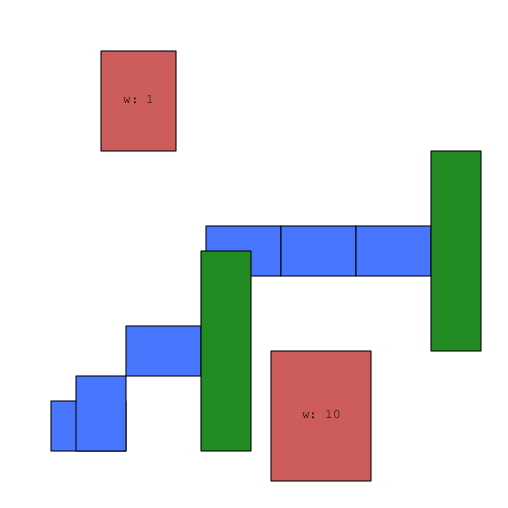
\includegraphics[width=0.5\textwidth]{feasible_world}
    \caption{Common Feasible World}
    \label{fig:feasible_world}
\end{figure}

\begin{table}[h!]
\centering
\begin{tabular}{@{}llllll@{}}
\toprule
Algorithm & Success(\%)  & Failure Time  & Success Time  & Path Length & Cover\\ 
\midrule
MCR & 100 & 0.00 & 34.287 & 5460.661 & 2.38 \\
RRT & 19 & 3.95 & 2.48 & 5561.92 & 0.0 \\ 
Bidirectional RRT & 100 & 0.00 & 0.96 & 5432.94 & 0.0 \\
Greedy IOR-RRT & 100 & 0.00 & 0.79 & 5116.33 & 1.4 \\
Probabilistic IOR-RRT & 100 & 0.00 & 0.83 & 5099.30 & 2.8 \\
Direct Trajectory & 100 & 0.00 & 0.04 & 3044.89 & 10 \\
Repeated IOR-RRT & 100 & 0.00 & 7.77 & 4653.65 & 0.0 \\
Search Informed IOR-RRT & 100 & 0.00 & 1.32 & 5400.34 & 0.0 \\
\bottomrule
\end{tabular}
\caption{Algorithm Performance on Minimal Obstacle World}
\label{tab:feasible_world}
\end{table}

The immediate observation is that despite being largely free space, the normal RRT regularly fails to find paths. Unsurprisingly the algorithms designed to find collision free paths when they exist (bidirectional RRT, search informed IOR-RRT) do find a collision free path on this planning problem. The repeated IOR-RRT has the same performance as measured by cover size, even though it is not designed to find minimal length covers; its success is the consequence of running an IOR-RRT more times than the normal IOR-RRTs resulting in more opportunities to find a good path. As expected, the direct trajectory performs poorly in the cover measure but excels in the time measure. The MCR algorithm however fails to find the true 0 cover MCR solution but also takes the most time of any algorithm.

\subsection{Cluttered World With Free Path}
In Figure \ref{fig:many_obstacles_feasible_world} we see a possible situation wherein a feasible path exists, but it is difficult to obtain. Table \ref{tab:many_obstacles_feasible_world} shows algorithm performance for this cluttered world.

\begin{figure}[h!]
    \centering
    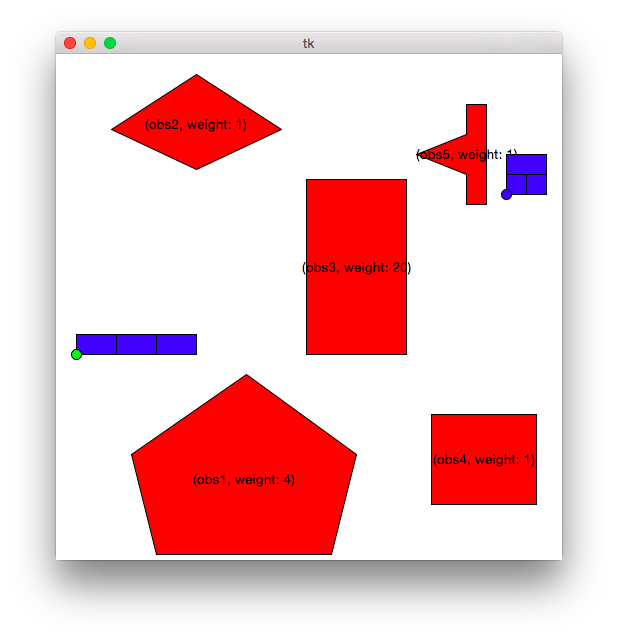
\includegraphics[width=0.5\textwidth]{many_obstacles_feasible_world}
    \caption{Cluttered Feasible World}
    \label{fig:many_obstacles_feasible_world}
\end{figure}


\begin{table}[h!]
\centering
\begin{tabular}{@{}llllll@{}}
\toprule
Algorithm & Success(\%)  & Failure Time  & Success Time  & Path Length & Cover\\ 
\midrule
MCR & 100 & 0.00 & 22.55 & 8161.90 & 2.34 \\
RRT & 3 & 2.76 & 2.28 & 7795.35 & 0 \\
Bidirectional RRT & 52 & 9.75 & 4.75 & 8676.26 & 0.00 \\
Greedy IOR-RRT & 100 & 0.00 & 2.94 & 9048.46 & 6.34 \\
Probabilistic IOR-RRT & 100 & 0.00 & 2.53 & 8693.80 & 11.54 \\
Direct Trajectory & 100 & 0.00 & 0.05 & 5154.62 & 21 \\
Repeated IOR-RRT & 100 & 0.00 & 25.11 & 8653.24 & 1.28 \\
Search Informed IOR-RRT & 100 & 0.00 & 9.79 & 9100.72 & 1.24 \\
\bottomrule
\end{tabular}
\caption{Algorithm Performance on Many Obstacles Feasible World}
\label{tab:many_obstacles_feasible_world}
\end{table}

By introducing a number of narrow hallways between obstacles, the motion planning problem has been made significantly more difficult for traditional motion planning techniques. Bidirectional RRT and RRT success fell to around 50\% and 3\%, respectively. Again, despite the true MCR solution being 0, the bounded time MCR still finds a path with a cover of 2 while taking 22 seconds to solve a single instance of the problem. The two IOR-RRT implementations find paths quickly in under 3 seconds. However, the cover of these two algorithms are high relative to $S^{*} = 0$. The greedy removal strategy outperforms the probabilistic removal strategy because of the impact that the induced randomness the sampling strategy adds. Since we use collision counts as measure of the value of a removal, a sampling strategy across this distribution can result in selecting obstacles for removal that are "wrong" (not optimal leading to overall higher cover scores). The repeated probabilistic removal IOR-RRT gets close to the true MCR solution for the reason described in the previous world experiment in addition to the repeated iterations giving the algorithm the opportunity to select the "right" obstacle to remove. 

The search informed IOR-RRT has some interesting behavior on this world. It succeeds in finding the lowest average cover due to its repeating the birrt search many times in its first phase. This helps it frequently find a collision-free path. Moreover, when it fails, because there does exist a collision-free path, it has been able to explore the space mitigating the number of obstacles it needs to remove to succeed unlike the normal IOR-RRTs.


\section{Worlds with Nonexistent Collision Free Paths}\label{results:unfeasible}
This section is used to analyze worlds where no feasible path exists. While these types of worlds are in the minority of planning problems a planner will face, it should be robust to these more rare circumstances. 

\subsection{Two Block World}
We start our analysis on unfeasible worlds with a simple analog to the minimal obstacle feasible world example from Figure \ref{fig:feasible_world}. The variant can be seen in Figure \ref{fig:two_soda_world}.

\begin{figure}[h!]
    \centering
    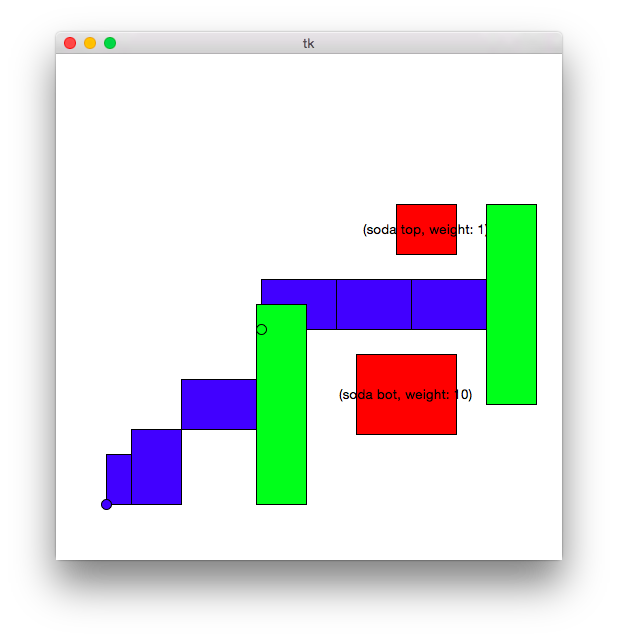
\includegraphics[width=0.5\textwidth]{two_soda_world}
    \caption{Two Box Unfeasible World}
    \label{fig:two_soda_world}
\end{figure}

\begin{table}[h!]
\centering
\begin{tabular}{@{}llllll@{}}
\toprule
Algorithm & Success(\%)  & Failure Time  & Success Time  & Path Length & Cover\\ 
\midrule
MCR & 100 & 0.00 & 12.58 & 6060.29 & 1.10 \\
RRT & 0 & 0.83 & 0.00 & 0.00 & 0.00 \\
Bidirectional RRT & 0 & 4.31 & 0.00 & 0.00 & 0.00 \\
Greedy IOR-RRT & 100 & 0.00 & 1.40 & 5151.30 & 2.00 \\
Probabilistic IOR-RRT & 100 & 0.00 & 1.36 & 5076.79 & 2.57 \\
Direct Trajectory & 100 & 0.00 & 0.04 & 3044.89 & 11.00 \\
Repeated IOR-RRT & 100 & 0.00 & 14.06 & 5221.01 & 1.00 \\
Search Informed IOR-RRT & 100 & 0.00 & 18.60 & 5538.52 & 1.45 \\
\bottomrule
\end{tabular}
\caption{Algorithm Performance on Two Block Unfeasible World}
\label{tab:two_soda_world}
\end{table}

Because the RRT and Bidirectional RRT search strategies only work in feasible worlds, it is natural that these two algorithms fail in this world. For the other worlds that are unfeasible, we will omit their performance since they necessarily fail. The optimal path cover in this example is a cover of weight one.  We note that in this unfeasible world with only two obstacles, the MCR algorithm takes around 13 seconds before returning a path with a good cover. This has to do with the fundamental MCR algorithm issue of not knowing when to return the found path (since it looks for iteratively better paths than a single, first path). 

The RRT variant algorithms we propose perform similarly. The directo trajectory, however, finds a path that collides with the top and bottom blocks (can be seen visually as well). Search informed IOR-RRTs outperform any of the basic IOR-RRT options but is outperformed by the repeated IOR-RRT. Additionally there is minimal impact on path lengths from any of the search-based algorithms.

\subsection{Cluttered World with Greedy Minimum Cover Path} \label{res:cluttered_world}
Here we examine the performance of the algorithms on worlds where the best cover paths exist through the direct path from the start to the goal. We would like to understand how the performance of our algorithms changes with the not only the number of obstacles but the location of the best paths.

\begin{figure}[h!]
    \centering
    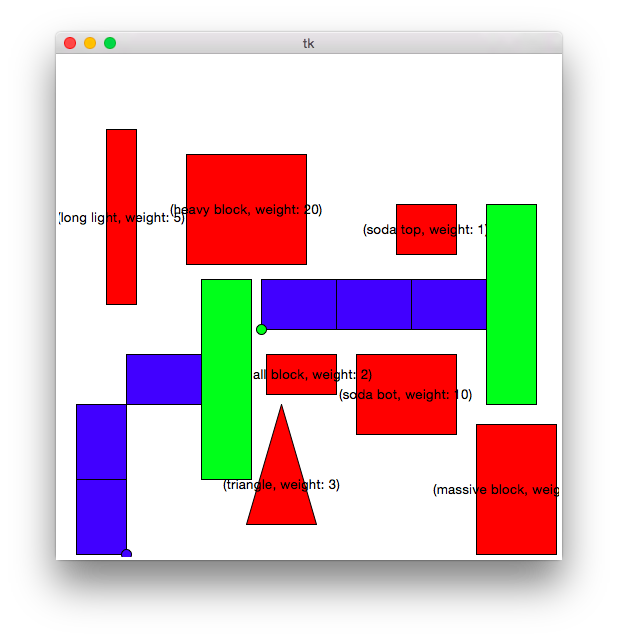
\includegraphics[width=0.5\textwidth]{cluttered_world}
    \caption{Cluttered World With Greedy Path of Minimum Cover}
    \label{fig:cluttered_world}
\end{figure}

\begin{table}[h!]
\centering
\begin{tabular}{@{}llllll@{}}
\toprule
Algorithm & Success(\%)  & Failure Time  & Success Time  & Path Length & Cover\\ 
\midrule
MCR & 100 & 0.00 & 118.69 & 4891.49 & 19.04 \\
Greedy IOR-RRT & 100 & 0.00 & 4.11 & 4656.24 & 16.30 \\
Probabilistic IOR-RRT & 100 & 0.00 & 5.36 & 4927.45 & 20.09 \\
Direct Trajectory & 100 & 0.00 & 0.09 & 3597.09 & 36.00 \\
Repeated IOR-RRT & 100 & 0.00 & 52.81 & 4617.88 & 15.96 \\
Search Informed IOR-RRT & 100 & 0.00 & 29.50 & 4576.64 & 16.80 \\
\bottomrule
\end{tabular}
\caption{Algorithm Performance on Cluttered World (With Greedy MCR Path)}
\label{tab:cluttered_world}
\end{table}

Again in Table \ref{tab:cluttered_world} we see that the MCR algorithm suffers heavily from a long running time. This high running time is partially a result of the MCR algorithm being one directional. Even if the $k$ frontier is high enough to find $S^*$, it may not succeed at finding the right connections to build the path resulting in a high cover. Since we use a version of MCR where the exit condition is based on the iteration number relative to the best cover found, the number of iterations we must run stays high causing a higher computation time. Additionally because the obstacle weights are widely distributed the algorithm spends a lot of time searching frontiers that cannot yield better path covers. The MCR algorithm's performance is tied to the size of the cover rather than the number of obstacles in the world, which is a problem in worlds with relatively few obstacles but with different weights. Unfortunately this is the more common scenario.

The greedy IOR-RRT finds paths with good covers as would be expected from the best path being a greedy path. Since goal biasing encourages both trees to grow towards each other, it would induce collisions with obstacles in the direct path from the start to the goal. Then the greedy removal strategy would select these obstacles for removal and a good path cover would be found. It is also clear then that the probabilistic removal strategy would lead to on average higher cover paths because it may deviate from the clear greedy path. The search informed algorithms perform the same from a cover perspective as the greedy removal IOR-RRT. Since the space is filled by obstacles, without removing any obstacles there is little space that the search strategy can fill in. Additionally the search informed RRT faces a big penalty in time performance because there does not exist a collision free path; the repeated attempts at looking for collision free paths without gaining additional information incurs no benefits at the expense of time.


\subsection{Cluttered World with Non-Greedy Minimum Cover Path}
In this last test we use a world that has the same layout as the previous world but with shifted obstacle weights such that the minimum cover path is no longer greedy but follows the top and left edges. 

\begin{figure}[h!]
    \centering
    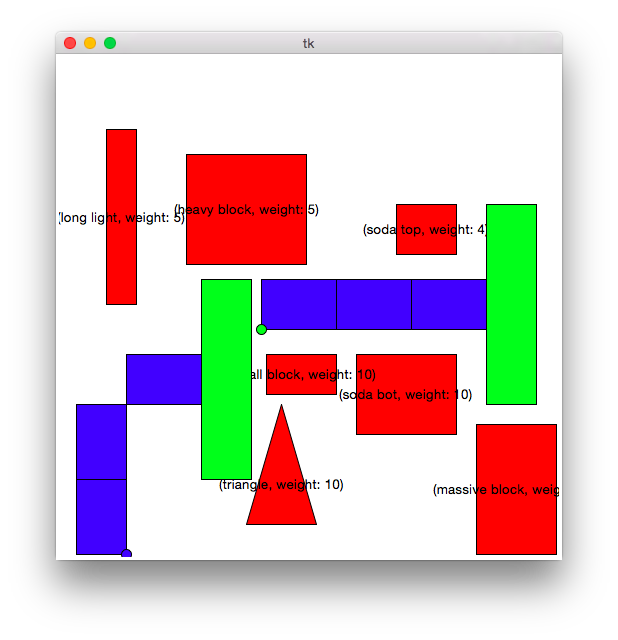
\includegraphics[width=0.5\textwidth]{top_light_cluttered_world}
    \caption{Cluttered World With Non-Greedy Path Of Minimum Cover}
    \label{fig:top_light_cluttered_world}
\end{figure}

\begin{table}[h!]
\centering
\begin{tabular}{@{}llllll@{}}
\toprule
Algorithm & Success(\%)  & Failure Time  & Success Time  & Path Length & Cover\\ 
\midrule
MCR & 100 & 0.00 & 163.32 & 6789.82 & 22.43 \\
RRT & 0 & 0.93 & 0.00 & 0.00 & 0.00 \\
Bidirectional RRT & 0 & 4.58 & 0.00 & 0.00 & 0.00 \\
Greedy IOR-RRT & 100 & 0.00 & 4.10 & 5189.46 & 25.15 \\
Probabilistic IOR-RRT & 100 & 0.00 & 5.45 & 5412.72 & 24.28 \\
Direct Trajectory & 100 & 0.00 & 0.09 & 3597.09 & 39.00 \\
Repeated IOR-RRT & 100 & 0.00 & 50.29 & 5860.71 & 14.75 \\
Search Informed IOR-RRT & 100 & 0.00 & 29.78 & 5386.64 & 27.00 \\
\bottomrule
\end{tabular}
\caption{Algorithm Performance on Cluttered World (With Non-Greedy MCR Path)}
\label{tab:top_light_cluttered_world}
\end{table}

We see that the greedy removal IOR-RRT is slightly outperformed by the probabilistic removal IOR-RRT. Since the ideal path is no longer along the greedy path from start to goal, the probabilistic removal strategy can succeed at opening up the middle space that the greedy removal strategy will not. Additionally, for the reasons mentioned in \ref{res:cluttered_world}, the first phase of the search informed IOR-RRT does not yield any benefit. The repeated IOR-RRT excels in this world due to the repeated chance to find good paths by opening the right space. Similar to the last world, MCR takes significantly longer than the other algorithms with the repeated IOR-RRT next. While the repeated IOR-RRT finds a cover of almost half the size as the search informed IOR-RRT, it takes 69\% longer than the search informed IOR-RRT, which itself takes notable time. 

\section{Discussion on Memory Factor Impact}
This section is dedicated to the impact of the memory factor on the IOR-RRT. Specifically we test the impact using the greedy removal IOR-RRT as the greedy removal strategy generally outperformed the probabilistic removal strategy evidenced by sections \ref{results:feasible}-\ref{results:unfeasible}. We use all memory factors in [0.0, 0.1, 0.3, 0.5, 0.7, 0.9, 1.0].

\begin{table}[h!]
\centering
\begin{tabular}{@{}llll@{}}
\toprule
Memory Factor & Two Block World(\%)  & Cluttered Greedy Path  & Cluttered Non-Greedy Path \\ 
\midrule
0.0 & 1.80 & 16.21 & 25.10 \\
0.1 & 1.74 & 16.09 & 25.16 \\
0.3 & 1.54 & 16.34 & 25.50 \\
0.5 & 1.78 & 16.92 & 25.51 \\
0.7 & 1.76 & 17.50 & 25.31 \\
0.9 & 2.00 & 19.51 & 25.35 \\ 
1.0 & 1.96 & 21.08 & 25.07 \\
\bottomrule
\end{tabular}
\caption{Covers Found by Greedy Removal IOR-RRT}
\label{tab:memory_factor_no_impact}
\end{table}

For all memory factors on all the worlds in Table \ref{tab:memory_factor_no_impact}, the greedy removal IOR-RRT had 100\% success rate. Moreover by inspection we see that there is no clear winner in which memory factor leads to the lowest found cover. Specifically the memory factor has negligible impact on the cover of the paths found. 

However, under certain conditions the memory factor can have an impact on the IOR-RRT's ability to find paths. Consider the example world in Figure \ref{fig:memory_factor_world} and the results of using the greedy removal IOR-RRT in Table \ref{tab:memory_factor_impact}.


\begin{figure}[h!]
    \centering
    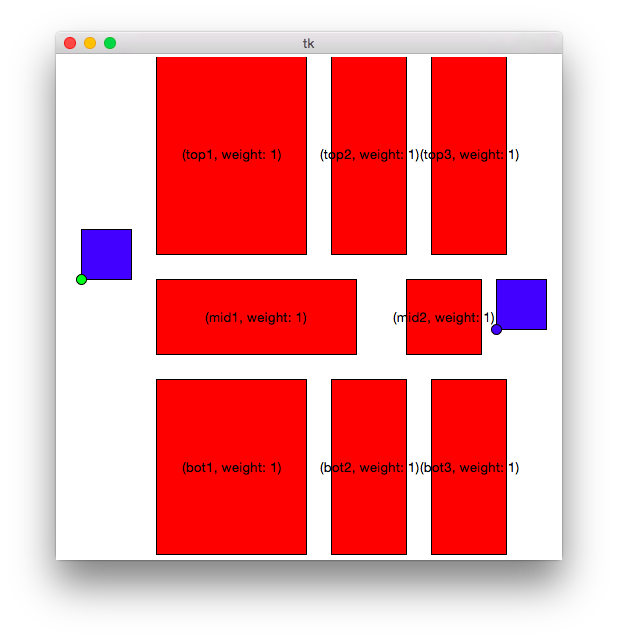
\includegraphics[width=0.5\textwidth]{memory_factor_world}
    \caption{World with Close Clustered Obstacles}
    \label{fig:memory_factor_world}
\end{figure}

\begin{table}[h!]
\centering
\begin{tabular}{@{}lllll@{}}
\toprule
Memory Factor & Success Rate(\%)  & Success Time & Path Length & Cover \\ 
\midrule
0.0 & 73.6 & 1.16 & 2223.69 & 2.35 \\
0.1 & 69.6 & 0.98 & 2201.90 & 2.39 \\
0.3 & 61.4 & 0.94 & 2188.36 & 2.27 \\
0.5 & 51.2 & 0.80 & 2153.86 & 2.21 \\
0.7 & 43.4 & 0.69 & 2176.99 & 2.18 \\
0.9 & 28.4 & 0.56 & 2216.65 & 2.17 \\ 
1.0 & 24.4 & 0.40 & 2190.09 & 2.18 \\
\bottomrule
\end{tabular}
\caption{World with Memory Factor Impact}
\label{tab:memory_factor_impact}
\end{table}

We see that low memory factors are correlated with success in finding paths in some situations. Low memory factors lead to higher rates of path discovery because it biases the planner to removing obstacles that are now exposed to collisions in the opened space. With a low removal frequency, collisions are accumulated for a longer period of time. Then, after removing an obstacle and scaling the collision counts by the memory factor, with a high memory factor there may still be a substantial collision count for the other obstacles that were in collision. Consequently the next removal cycle may select one of those original obstacles for removal. Holding the number of removals constant, this can be a wasted obstacle removal. 

In the case of Figure \ref{fig:memory_factor_world}, collisions are many times evenly split among obstacles "mid1" and "top1". This results in, with a high memory factor, both obstacles being removed rather than just one of them. Since there aren't enough removal cycles to remove sufficient obstacles after removing both of these obstacles, no path is found, leading to the lower success rate. This then motivates using 0 memory factor and restarting our counting of collisions after every removal. Funamentally, this is the correct choice as we are interested in quickly finding a path from a start configuration to a goal configuration using collision counts as a measure of importance. After picking an obstacle we have claimed that this obstacle is the correct choice and the others are "wrong". This suggests that we should favor exploring new space instead of reducing risk by keeping old memory. This is epecially true when the speed and success at finding a path is more valuable than a more correct path and possibly no path.



\chapter{Conclusion}
In this research paper we examined existing techniques for motion planning like the RRT, the bidirectional RRT, and MCR. We propose the IOR-RRT, the repeated IOR-RRT, and the search informed IOR-RRT. We are interested in algorithms that are robust to the presence of feasible paths in planning problems.

Traditional motion planning techniques do not satisfy this requirement since they are not suited to unfeasible planning problems. Additionally, we have shown that MCR often underperforms in bounded iterations by taking a long time to find subpar paths as measured by covers. Amongst the algorithms in Chapter \ref{chap:algos}, we see that the direct trajectory is the worst in all scenarios. Between the IOR-RRT and search informed IOR-RRT, the search informed RRT is more likely to find collision free paths when they exist, suggesting that the correct choice is to use the latter because the cost of finding paths with collisions when collision free paths exist is high in the planning process. The greedy removal strategy empirically outperforms the probabilistic removal strategy in cover score. The greedy removal strategy can also yield a higher success rate when the number of constraint removals allowed (specified by the removal frequency) is close to the number of constraint removals done with greedy removal, which is lower bounded by the true number of constraint removals needed.

The choice between the search informed IOR-RRT with greedy removal and the repeated IOR-RRT with probabilistic removal centers around computation time. We saw that in complicated unfeasible worlds with many obstacles, the repeated IOR-RRT could find paths with better covers at the cost of taking almost 85\% longer to return a path. However, the repeated IOR-RRT only finds significantly better covers when the MCR solution is along a non-greedy path from the start configuration to the goal configuration. In feasible worlds, which are the most common, the search informed IOR-RRT is much faster at finding a good path. Between the two options, the search informed IOR-RRT provides the best tradeoff of computation time and good path covers.

The search informed iterative obstacle removing RRT with greedy removal is the best choice for use in a planner. While it does not always find a path with the lowest cover, it instead offers an algorithm that can find collision free paths when possible and otherwise quickly find reasonably good paths. This strategy can be used in planners that must be able to identify mechanisms for making actions feasible.
\appendix
%\chapter{Tables}

\begin{table}
\caption{Armadillos}
\label{arm:table}
\begin{center}
\begin{tabular}{||l|l||}\hline
Armadillos & are \\\hline
our	   & friends \\\hline
\end{tabular}
\end{center}
\end{table}

\clearpage
\newpage

%\chapter{Figures}

\vspace*{-3in}

\begin{figure}
\vspace{2.4in}
\caption{Armadillo slaying lawyer.}
\label{arm:fig1}
\end{figure}
\clearpage
\newpage

\begin{figure}
\vspace{2.4in}
\caption{Armadillo eradicating national debt.}
\label{arm:fig2}
\end{figure}
\clearpage
\newpage

%% This defines the bibliography file (main.bib) and the bibliography style.
%% If you want to create a bibliography file by hand, change the contents of
%% this file to a `thebibliography' environment.  For more information
%% see section 4.3 of the LaTeX manual.
\begin{singlespace}
\bibliographystyle{mybib}
\bibliography{main}
\end{singlespace}

\listoftodos
\end{document}

